\appendix
\renewcommand\thesection{\Alph{section}}
\setcounter{section}{0}
\renewcommand\thefigure{S\arabic{figure}}
\setcounter{figure}{0}
\renewcommand\thetable{S\arabic{table}}
\setcounter{table}{0}
\renewcommand\theequation{S\arabic{equation}}
\setcounter{equation}{0}



\section{Data Processing Pipeline}
\label{sec:data_processing}

Training a general-purpose streaming 3D reconstruction model requires
large-scale, diverse data with accurate ground-truth camera poses and
depth maps. Our training corpus (Section~\ref{sec:training_data})
spans 29 datasets from heterogeneous sources, each with different
data formats, coordinate conventions, depth representations, and
quality characteristics. To unify these into a consistent training
pipeline, we develop a multi-stage data processing strategy:
(1)~\textit{Existing data processing} (\secref{sec:existing_data}):
standardizing publicly available datasets by converting
coordinate systems, normalizing depth scales, filtering corrupted
frames, and unifying metadata formats;
(2)~\textit{Synthetic data generation} (\secref{sec:gen_data}):
rendering additional training data from 3D environments with
controlled camera trajectories and pixel-perfect ground truth;
(3)~\textit{Gaming data processing} (\secref{sec:gaming_data}):
extracting high-quality pose and depth annotations from internal
game engine captures, which provide long trajectories through
large-scale, visually rich environments;
(4)~\textit{MatrixCity data sequencing} (\secref{sec:matrixcity_data}):
reorganizing the MatrixCity aerial and street-level data into
temporally continuous sequences via random walks on spatial
topologies, enabling its use for sequential training;
(5)~\textit{Cross-scene traversal data} (\secref{sec:traversal_data}):
rendering long-range cross-room RGBD video sequences from
large-scale 3D scene reconstructions using Habitat-Sim, providing
the multi-room traversal signals that existing indoor datasets lack.
Below we describe each pipeline in detail.

\subsection{Existing Data Processing}
\label{sec:existing_data}
To facilitate multi-dataset training, we standardize all 29 publicly available datasets into a unified format through a series of preprocessing steps.

\textbf{Coordinate System Unification.} Datasets store camera poses using different
conventions.  We convert all poses to a consistent camera to world representation.
For datasets with non-standard axis conventions, such as UnReal4K~\cite{tosi2021smd},  an additional rotation matrix is applied to align the coordinate system with the OpenCV standard. Intrinsic parameters are either extracted from per-frame calibration files (\eg, .npz) or set to known constant values for datasets with a fixed camera model, such as TartanAir~\cite{wang2020tartanair}.

\textbf{Depth Scale Normalization.} The raw depth maps are provided in diverse formats and units. For instance, ScanNet and ScanNet++ store depth in millimeters as 16-bit PNG files, which are converted by dividing by 1000. VirtualKITTI2 uses centimeters stored in 16-bit color images, requiring division by 100. Other datasets, including DL3DV, HyperSim, TartanAir, and BlendedMVS, provide raw float .npy arrays in meters, while Waymo utilizes OpenEXR floating-point maps. All depth values are uniformly converted to meters and stored as float32.

\textbf{Corrupted Frame Filtering.} We apply several validation checks to remove corrupted or degenerate frames. First, scenes are discarded if the number of RGB images, depth maps, and camera pose files is inconsistent. Second, sequences with fewer than a minimum threshold of valid frames are excluded. Third, invalid depth values such as NaN or Inf are set to zero. Fourth, for datasets with noisy depth like DL3DV and MVS Synth, values exceeding the 98th percentile or an absolute threshold (\eg, 1000m) are clamped to zero. Fifth, for outdoor datasets such as DL3DV and Mapfree, sky regions are identified using pre-computed masks or depth saturation thresholds and their corresponding depth is set to zero. 
Finally, for DL3DV and Mapfree, pre-computed outlier masks are used to further remove geometrically inconsistent depth estimates. 

\textbf{Metadata Format Unification.} All datasets are converted into a common metadata structure, which is serialized as pickle files. This structure contains scene lists, per-frame index mappings (sceneids, id ranges), paths to images and depth maps, intrinsic matrices, and camera trajectories as 4$\times$4 pose matrices. This unified format is generated and cached during the initial execution, which enables efficient composition of multiple datasets at training time without requiring repeated parsing of the raw data.




\subsection{Generation Data Settings}
\label{sec:gen_data}

We render multi-view images of 3D assets in Objaverse~\cite{deitke2023objaverse} 
and Texverse~\cite{zhang2025texverse} using Blender Cycles. Each scene is normalized to fit within $[-0.9, 0.9]^3$. A pinhole camera with $\theta_h \sim \mathcal{U}(40^\circ, 70^\circ)$ and focal length $f = w / (2\tan(\theta_h/2))$ captures $512\times512$ images. Camera positions are sampled on a sphere around the origin at multiple elevations, all oriented toward the scene center. We apply HDR environment lighting and render RGBA color and metric depth in OpenEXR format. Images are tonemapped using percentile-based normalization with $\gamma{=}1/2.2$ correction.

\subsection{Gaming Data Processing Pipeline}
\label{sec:gaming_data}


\noindent We introduce a runtime acquisition pipeline that captures dense visual and geometric annotations from modern game engines. This provides a scalable source of large-scale, accurately annotated, and stylistically diverse long-sequence 3D data that is otherwise difficult to obtain from real-world captures alone. All sequences maintain high visual quality with smooth camera motion and sufficient inter-frame overlap, free of motion blur, over-exposure, or under-exposure artifacts. The dataset covers a wide variety of viewpoints including forward, lateral, and vertical gaze directions, and incorporates both intra-sequence and inter-sequence field-of-view variations to improve robustness to focal-length changes. Cutscenes, UI overlays, and other non-gameplay frames are excluded, and all graphics settings remain constant within each game to ensure consistent annotation quality across the entire dataset.

To ensure sufficient diversity in scene types and camera behaviors, we
establish a standardized collection protocol organized into two primary categories based on environment type:

\begin{itemize}
\item \textbf{Indoor scenes:} Covers navigation
  within enclosed environments such as buildings, rooms, and corridors.
  \begin{itemize}
  \item \textit{Free roaming:} Stochastic exploration along random
    trajectories, with frequent room transitions and floor changes;
  \item \textit{Loop roaming:} Departing from and returning to the same
    location to form closed-loop sequences through interconnected rooms;
  \item \textit{Transition navigation:} Traversing significant scene
    boundaries such as moving between distinct interiors or exiting to
    outdoor areas via doors and elevators.
  \end{itemize}

\item \textbf{Outdoor scenes:} Covers a broader
  range of navigation and observation modes in open environments.
  \begin{itemize}
  \item \textit{Free roaming:} Stochastic exploration along random
    trajectories, with diverse headings and frequent lateral viewpoint
    changes;
  \item \textit{Loop roaming:} Departing from and returning to the same
    location to form closed-loop sequences across open terrain;
  \item \textit{Transition navigation:} Traversing significant scene
    boundaries such as entering or exiting buildings and crossing between
    distinct outdoor regions;
  \item \textit{Dynamic sightseeing:} Touring scenes containing moving
    elements such as pedestrians, vehicles, or animals;
  \item \textit{Object orbiting:} Circling around objects to
    capture multi-view observations.
  \end{itemize}
\end{itemize}

\subsection{MatrixCity Data Sequencing}
\label{sec:matrixcity_data}

The MatrixCity dataset provides aerial and street-level multi-view images with known camera poses. However, the original data is organized for spatial coverage rather than temporal continuity---aerial images are sampled on a regular grid, while street images are stored as independent road segments. This is incompatible with downstream tasks that require temporally continuous input, such as video generation and sequential 3D reconstruction. We reorganize both data types into view-continuous sequences by performing random walks on their respective spatial topologies, without modifying the original images or poses.

\subsubsection{Aerial Data}
\label{sec:aerial_data}

\paragraph{Data layout.}
Aerial data is arranged on an $H\!\times\!W$ regular grid in row-major order (\cref{fig:aerial}\,a). Each scene may contain multiple \emph{grid loops}, each corresponding to a complete grid sampling pass. The frame index~$i$ and grid coordinate $(r,c)$ satisfy
\begin{equation}
  r = \lfloor i / W \rfloor, \quad c = i \bmod W.
  \label{eq:grid_index}
\end{equation}
Consecutive frames are row-wise neighbors on the grid, but spatial discontinuities occur at row boundaries (\eg, the last frame of one row and the first frame of the next row are far apart), so the raw storage order does not form a natural camera trajectory.

\paragraph{Sequencing method.}
We treat the grid as a graph with 8-connected adjacency and perform random walks to produce spatially continuous trajectories (Fig.~\ref{fig:aerial}\,b). To suppress immediate backtracking, each step excludes the previous position from the candidate set. Grid coordinates are mapped to global frame indices via
\begin{equation}
  \mathrm{idx} = l \cdot N_{\mathrm{loop}} + r \cdot W + c,
  \label{eq:global_index}
\end{equation}
where $l$ is the grid loop index and $N_{\mathrm{loop}}$ is the number of frames per loop. The number of sequences is proportional to the data size (by default, 5 sequences per 1{,}000 frames). The full procedure is given in Algorithm~\ref{alg:aerial}.

\begin{figure}[t]
  \centering
  \begin{subfigure}[t]{0.48\linewidth}
    \centering
    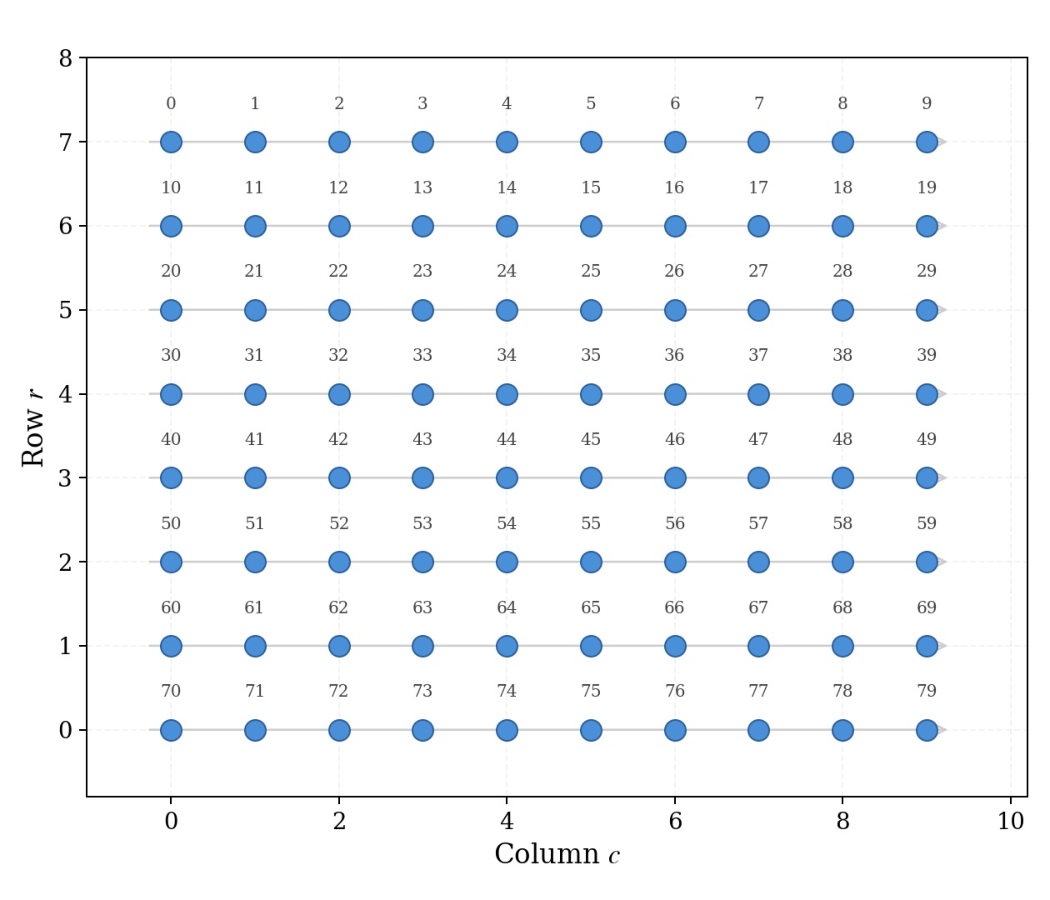
\includegraphics[width=\linewidth]{figures/matrixcity/fig_aerial_grid.pdf}
    \caption{Row-major grid layout.}
    \label{fig:aerial_grid}
  \end{subfigure}
  \hfill
  \begin{subfigure}[t]{0.48\linewidth}
    \centering
    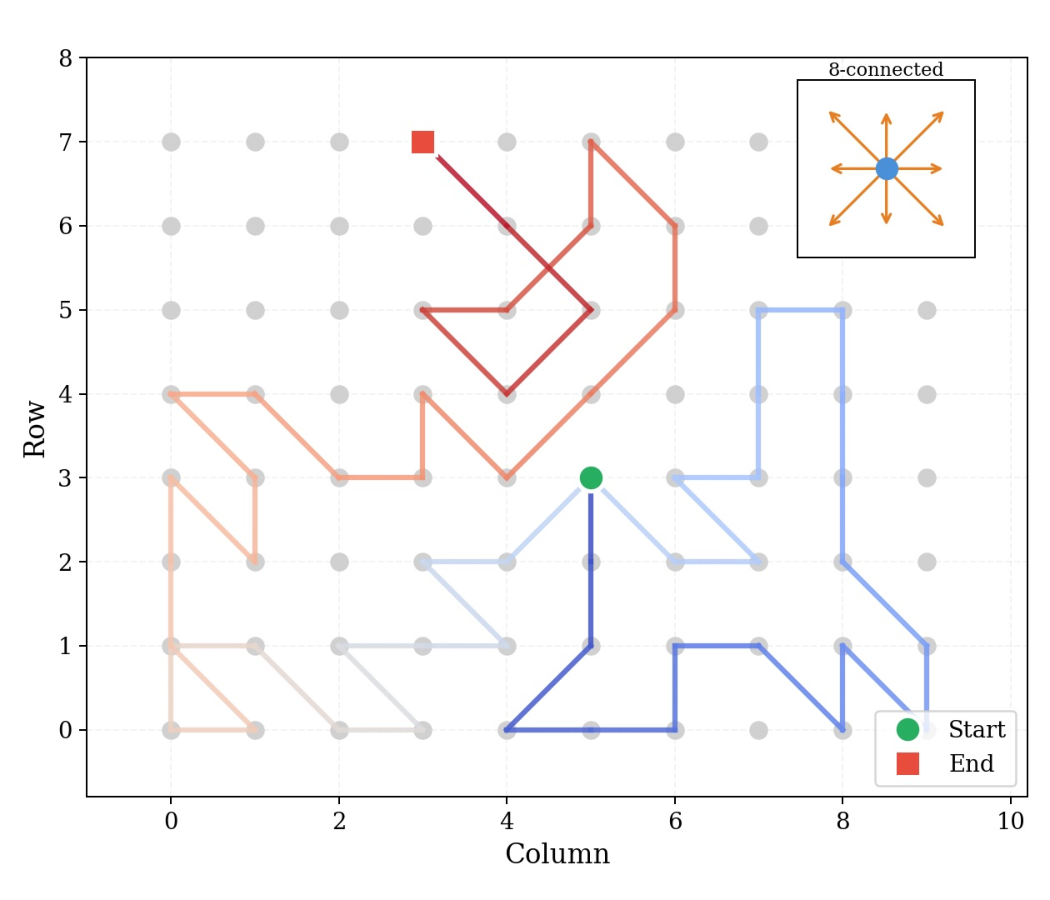
\includegraphics[width=\linewidth]{figures/matrixcity/fig_aerial_walk.pdf}
    \caption{8-connected random walk.}
    \label{fig:aerial_walk}
  \end{subfigure}
  \caption{Aerial data sequencing. \textbf{(a)}~Each blue node is a camera position labeled by its row-major index ($\mathrm{index} = r \times W + c$); gray arrows show the storage scan order. \textbf{(b)}~A random walk on the grid; color gradient (blue $\to$ red) encodes temporal progression. The inset shows the 8-connected neighborhood. Each step excludes the previous position to suppress backtracking.}
  \label{fig:aerial}
\end{figure}

\begin{algorithm}[t]
\caption{Aerial Grid Random Walk}
\label{alg:aerial}
\begin{algorithmic}[1]
\Require Grid size $H\!\times\!W$, sequence length $T$, loop index $l$
\Ensure Frame index sequence $\mathcal{S}$
\State Sample random start position $(r, c) \in [0,H) \times [0,W)$
\State $\mathrm{prev} \gets \texttt{null}$
\For{$t = 1$ \textbf{to} $T$}
    \State $\mathcal{S}.\text{append}(l \cdot N_{\mathrm{loop}} + r \cdot W + c)$
    \State $\mathcal{N} \gets \{(r\!+\!\Delta r,\, c\!+\!\Delta c) \mid (\Delta r, \Delta c) \in \mathcal{D}_8\} \cap \mathcal{G} \;\setminus\; \{\mathrm{prev}\}$
    \If{$\mathcal{N} = \emptyset$}
        \State $\mathcal{N} \gets$ all valid 8-connected neighbors \Comment{corner fallback}
    \EndIf
    \State $\mathrm{prev} \gets (r, c)$
    \State $(r, c) \gets \textsc{RandomChoice}(\mathcal{N})$
\EndFor
\State \Return $\mathcal{S}$
\end{algorithmic}
\end{algorithm}

\subsubsection{Street Data}
\label{sec:street_data}

\paragraph{Data layout.}
Street data is captured per-street. Each street is a linear trajectory with $N$ evenly-spaced camera positions, each photographed from 5 viewpoints (viewpoints 0--3 are horizontal; viewpoint~4 is zenith-facing), yielding $5N$ frames per street. Frames are stored in viewpoint-first order: all $N$ positions of viewpoint~0 appear first, followed by viewpoints 1--4 in sequence. Different streets may physically intersect (\eg, at crossroads), but are stored independently without explicit connectivity information.

Sequencing proceeds in three stages (\cref{fig:street}): street identification, intersection detection, and graph-based random walk.

\paragraph{Stage 1: Street identification.}
We exploit the viewpoint-first storage order to automatically segment street boundaries via \emph{position repetition detection} (\cref{fig:street}\,a). Frames are traversed sequentially, and camera positions are extracted. A set of unique positions $\mathcal{U}$ is maintained; when a new position falls within $\epsilon = 0.01$\,m of any existing point in $\mathcal{U}$, it is flagged as a duplicate, indicating that viewpoint~0 traversal is complete. At this point $|\mathcal{U}| = N$ gives the number of unique positions for that street, and the subsequent $5N$ frames are partitioned into 5 viewpoint segments.

\paragraph{Stage 2: Intersection detection and graph construction.}
To establish topological connectivity, each street is simplified to its endpoint-to-endpoint 2D line segment (projected onto the $XY$ plane), and all segment pairs are tested for intersection (\cref{fig:street}\,b). To handle streets that are physically close but do not precisely intersect (\eg, T-junctions), each segment is optionally extended by a configurable distance $d_{\mathrm{ext}}$ at both ends before testing. Detected intersections define an undirected street connectivity graph $G = (V, E)$, where vertices~$V$ are streets and edges~$E$ connect intersecting pairs.

\paragraph{Stage 3: Graph-based random walk.}
We generate cross-street continuous sequences by performing random walks on $G$ (\cref{alg:street},~\cref{fig:street}\,c). Three key design choices ensure sequence quality:
\begin{enumerate}[leftmargin=*,nosep]
  \item \textbf{Intersection decisions.} When the walker approaches an intersection (distance $< d_{\mathrm{prox}}$), it switches to a connecting street with probability $p_{\mathrm{turn}} = 0.5$.
  \item \textbf{Viewpoint continuity.} Upon switching streets, the viewpoint whose camera forward direction (third column of the rotation matrix) best matches the current one is selected:
  \begin{equation}
    v^* = \arg\max_{v \in \{0,\dots,4\}} \; \mathbf{f}_{\mathrm{curr}} \cdot \mathbf{f}_{v}.
    \label{eq:viewpoint_select}
  \end{equation}
  \item \textbf{Endpoint handling.} At dead ends (degree $\leq 1$), the walking direction is reversed.
\end{enumerate}

\begin{figure}[t]
  \centering
  \begin{subfigure}[t]{0.32\linewidth}
    \centering
    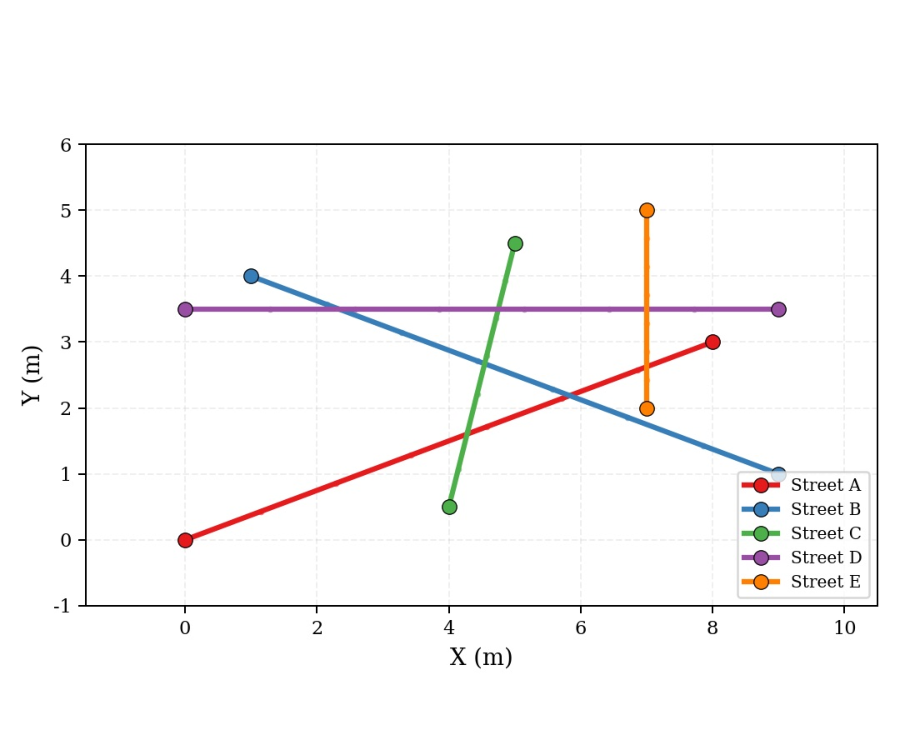
\includegraphics[width=\linewidth]{figures/matrixcity/fig_street_stage1.pdf}
    \caption{Street identification.}
    \label{fig:street_stage1}
  \end{subfigure}
  \hfill
  \begin{subfigure}[t]{0.32\linewidth}
    \centering
    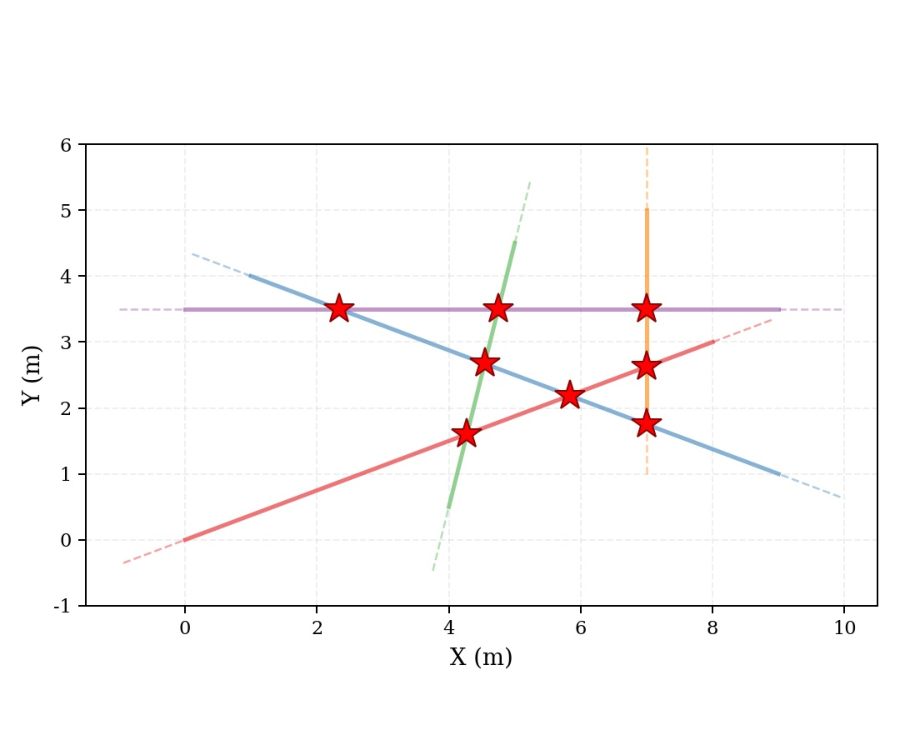
\includegraphics[width=\linewidth]{figures/matrixcity/fig_street_stage2.pdf}
    \caption{Intersection detection.}
    \label{fig:street_stage2}
  \end{subfigure}
  \hfill
  \begin{subfigure}[t]{0.32\linewidth}
    \centering
    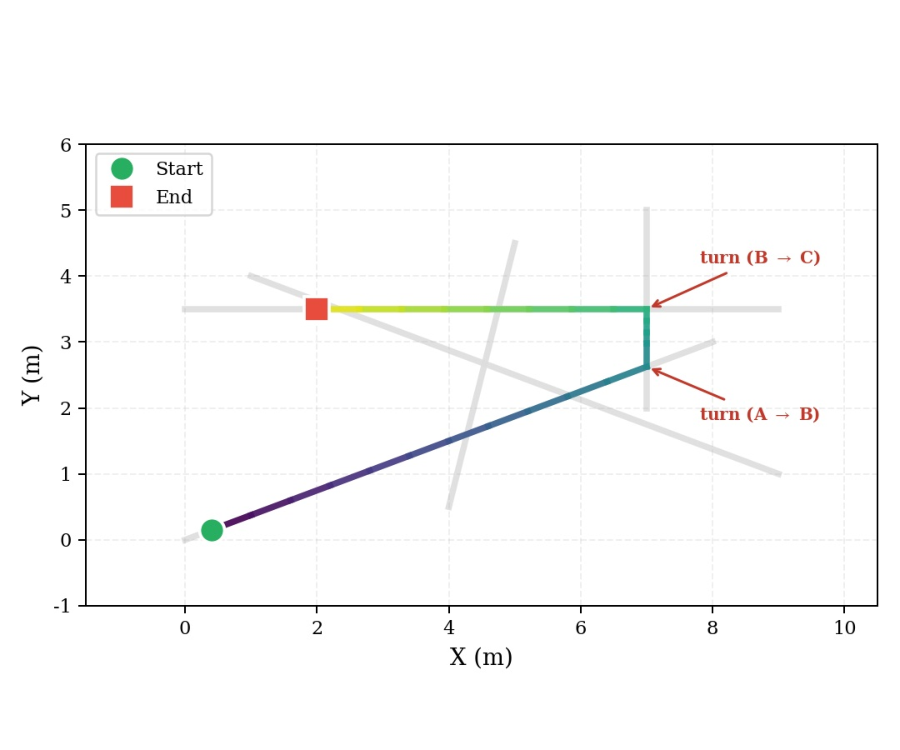
\includegraphics[width=\linewidth]{figures/matrixcity/fig_street_stage3.pdf}
    \caption{Graph-based random walk.}
    \label{fig:street_stage3}
  \end{subfigure}
  \caption{Street data sequencing pipeline. \textbf{(a)}~Stage~1: independently identified street segments (A--E) with camera positions (dots). \textbf{(b)}~Stage~2: red stars mark detected intersections; dashed lines show optional segment extensions for near-miss junctions. \textbf{(c)}~Stage~3: a random walk traversing Street~A $\to$ B $\to$ C via intersections; color gradient encodes temporal order.}
  \label{fig:street}
\end{figure}

\begin{algorithm}[t]
\caption{Street Network Random Walk}
\label{alg:street}
\begin{algorithmic}[1]
\Require Street graph $G$, sequence length $T$, turn probability $p_{\mathrm{turn}}$, proximity threshold $d_{\mathrm{prox}}$
\Ensure Frame sequence $\mathcal{S}$
\State Randomly select start street $e$, position index $i$, viewpoint $v \in \{0..3\}$, direction $d \in \{+1, -1\}$
\For{$t = 1$ \textbf{to} $T$}
    \State $\mathcal{S}.\text{append}\bigl(\textsc{Frame}(e, i, v)\bigr)$
    \State $i_{\mathrm{next}} \gets i + d$
    \If{$i_{\mathrm{next}}$ out of bounds} \Comment{street endpoint}
        \If{$\deg(e) \leq 1$}
            \State $d \gets -d$ \Comment{dead end: reverse}
        \Else
            \State $(e, i, v, d) \gets \textsc{SwitchStreet}(e, i, v)$
        \EndIf
    \ElsIf{$\exists$ intersection within $d_{\mathrm{prox}}$ \textbf{and} $\textsc{Rand}() < p_{\mathrm{turn}}$}
        \State $(e, i, v, d) \gets \textsc{SwitchStreet}(e, i, v)$
    \Else
        \State $i \gets i_{\mathrm{next}}$ \Comment{advance along current street}
    \EndIf
\EndFor
\State \Return $\mathcal{S}$
\Statex
\Function{SwitchStreet}{$e, i, v$}
    \State $e' \gets$ random neighbor of $e$ in $G$
    \State $i' \gets$ nearest position on $e'$ to intersection point
    \State $v' \gets \arg\max_{v''} \mathbf{f}_{\mathrm{curr}} \cdot \mathbf{f}_{v''}$ \Comment{viewpoint continuity}
    \State $d' \gets$ direction away from intersection
    \State \Return $(e', i', v', d')$
\EndFunction
\end{algorithmic}
\end{algorithm}





\subsection{Cross-Scene Traversal Data Construction}
\label{sec:traversal_data}

Long-range streaming 3D reconstruction requires the model to handle continuously expanding observation sequences in which the camera moves from one room through a corridor into the next, encountering substantial changes in geometry and appearance along the way. Existing indoor RGBD datasets (\eg, ScanNet~\cite{dai2017scannet}) are largely confined to single rooms or small regions and therefore lack the cross-region, long-range traversal signals needed for training. To address this limitation, we render cross-room continuous RGBD video sequences from large-scale real-world 3D scene reconstructions using Habitat-Sim~\cite{savva2019habitat}.

\paragraph{Scene sources.}
We draw scenes from three complementary indoor 3D datasets: Gibson~\cite{xia2018gibson} (${\sim}$450 building-scale scans covering residential and office environments with high geometric fidelity), Matterport3D~\cite{chang2017matterport3d} (90 large residential and commercial spaces, each typically containing 10 to 30 rooms with rich furniture layouts and multi-story structures), and HM3D~\cite{ramakrishnan2021hm3d} (900 semantically diverse indoor environments spanning a wide range of scene scales and complexities). The three datasets differ in capture devices, reconstruction quality, and scene types, and their joint use broadens the training distribution while mitigating overfitting to any single data source.

\paragraph{Trajectory generation.}
For each scene, we first compute a navigation mesh and then randomly sample $N{+}1$ waypoints on walkable surfaces, requiring a minimum geodesic distance of 2\,m between consecutive waypoints to ensure sufficient spatial coverage. The number of segments $N$ is drawn from a piecewise mixture distribution (40\% in 5 to 8, 45\% in 8 to 12, and 15\% in 12 to 16), corresponding to local exploration, cross-functional-area walking, and full-scene traversal, respectively. Adjacent waypoints are connected via the shortest geodesic path on the navigation mesh, allowing trajectories to naturally pass through doorways and corridors for cross-room traversal. The concatenated path is then linearly interpolated, smoothed with a double-pass moving average, and projected back onto the navigation mesh, yielding a dense, smooth, and physically plausible trajectory. A single trajectory typically comprises 500 to 3{,}000 frames (roughly 15 to 100\,s at 30\,fps).

\paragraph{Motion control.}
To produce realistic egocentric videos, we design a multi-stage motion controller that converts the trajectory path into per-frame camera poses. Translation is governed by a first-order low-pass filter ($\alpha{=}0.18$) combined with navigation-mesh collision correction. Yaw is steered toward a lookahead target 10 frames ahead through a $\tanh$-saturated velocity model that provides natural acceleration and deceleration during turns. Pitch follows terrain elevation changes and is smoothed by exponential decay. On top of this base motion, IIR-filtered Gaussian noise is added to both position and orientation to simulate handheld camera shake, and stochastic glance events, \ie brief lateral and vertical head turns following a half-cosine envelope, are triggered at random to reproduce the natural gaze shifts that occur during walking.

\paragraph{Parameter diversification.}
Camera intrinsics and motion parameters are independently sampled per sequence from piecewise mixture uniform distributions to cover a broad range of real-world conditions: horizontal field of view from 40\textdegree{} to 100\textdegree, sensor height from 1.35 to 1.80\,m, walking speed from 0.3 to 1.8\,m/s, and several tiers of jitter intensity and glance frequency. Walking speed is sampled independently per trajectory segment, producing natural speed variations within a single sequence. All randomized parameters and waypoint coordinates are recorded in a configuration file for exact reproducibility.

\paragraph{Rendering and output.}
We employ a pinhole camera model and render at $640{\times}480$ resolution and 30\,fps, producing per-frame RGB images and metric depth maps together with 6-DoF camera poses (position and quaternion) and intrinsics ($f_x, f_y, c_x, c_y$). In total, we generate approximately 2{,}800 sequences from the three datasets, each containing 1k to 5k frames, amounting to 14.4\,TB of data. \Cref{fig:traversal_viz} visualizes the top-down point clouds and sampled trajectories for several representative scenes.



\begin{figure*}[t]
  \centering
  \setlength{\tabcolsep}{1.5pt}
  \adjustbox{max width=\linewidth}{%
  \begin{tabular}{ccc}
    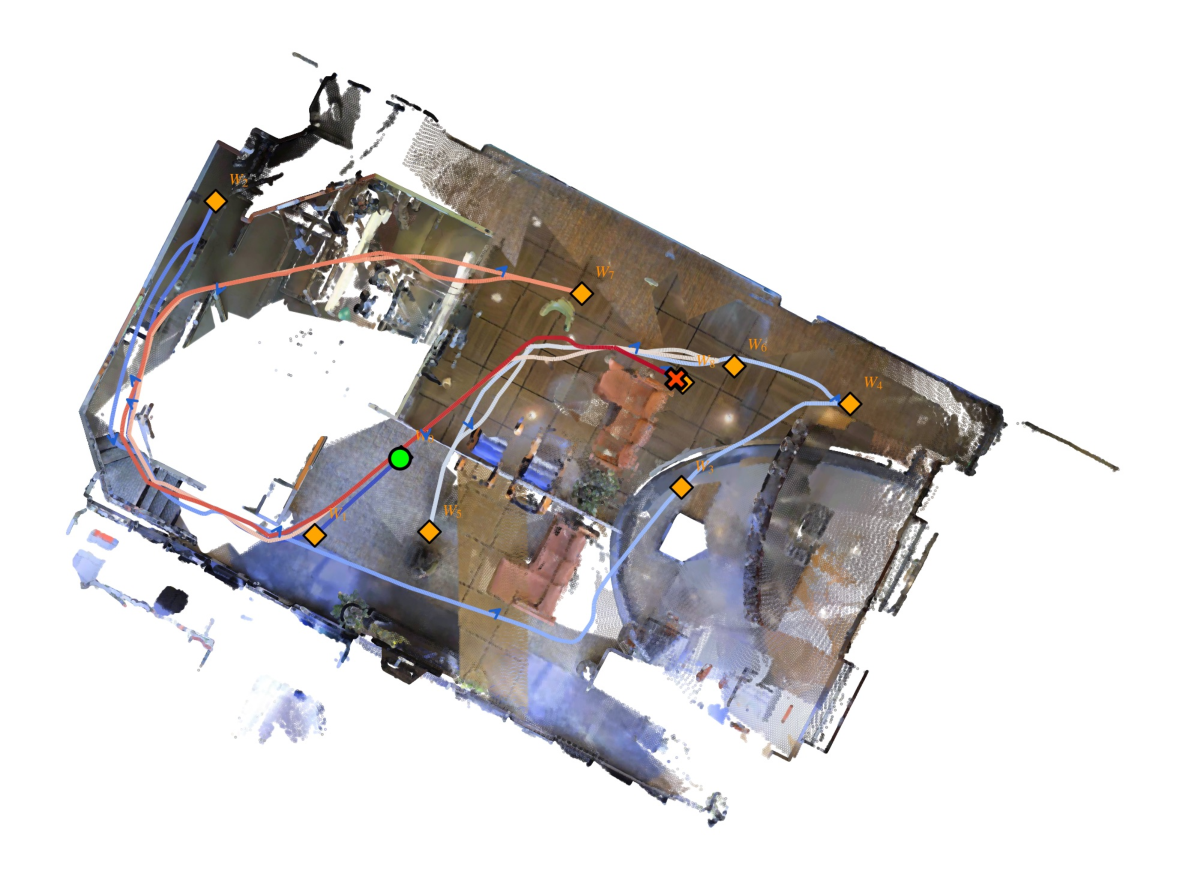
\includegraphics[height=0.2\linewidth]{figures/habitat/mp3d_1.pdf} &
    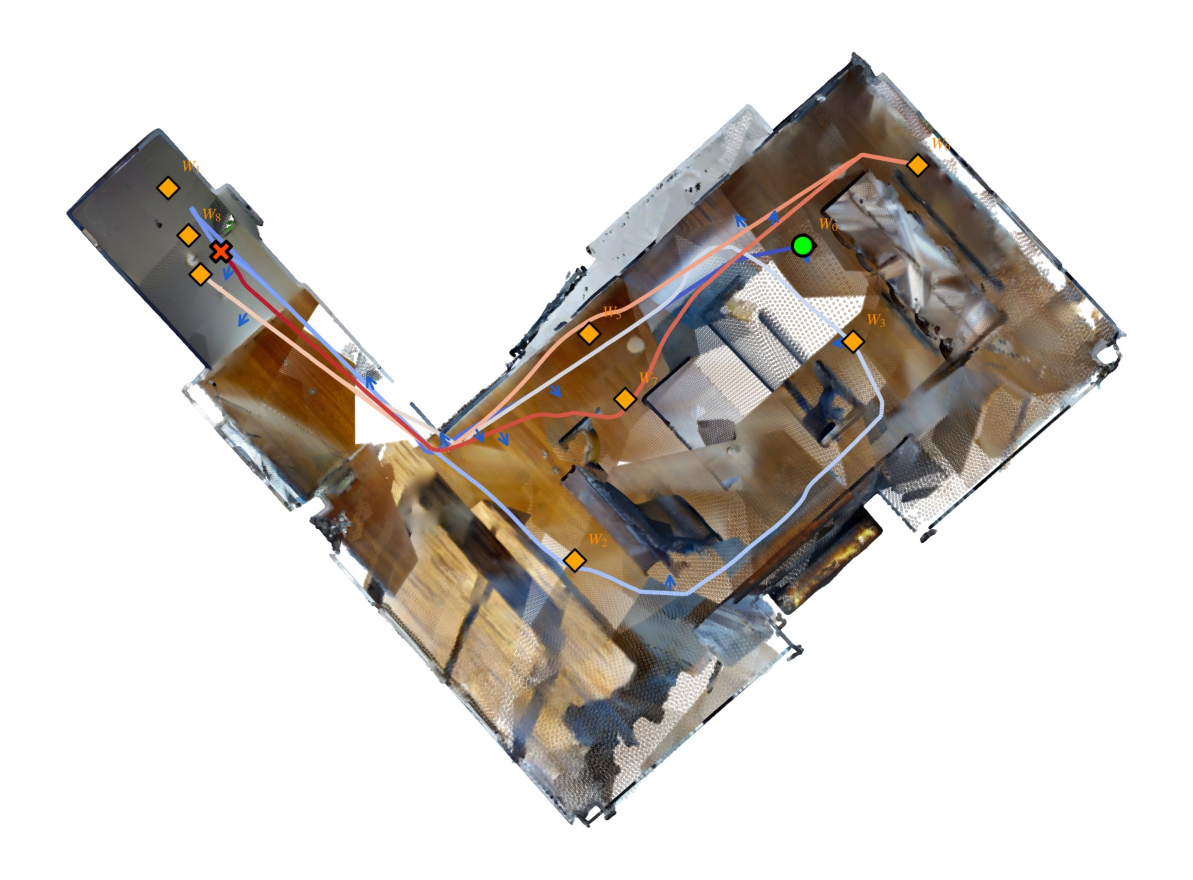
\includegraphics[height=0.2\linewidth]{figures/habitat/gibson_1.pdf} &
    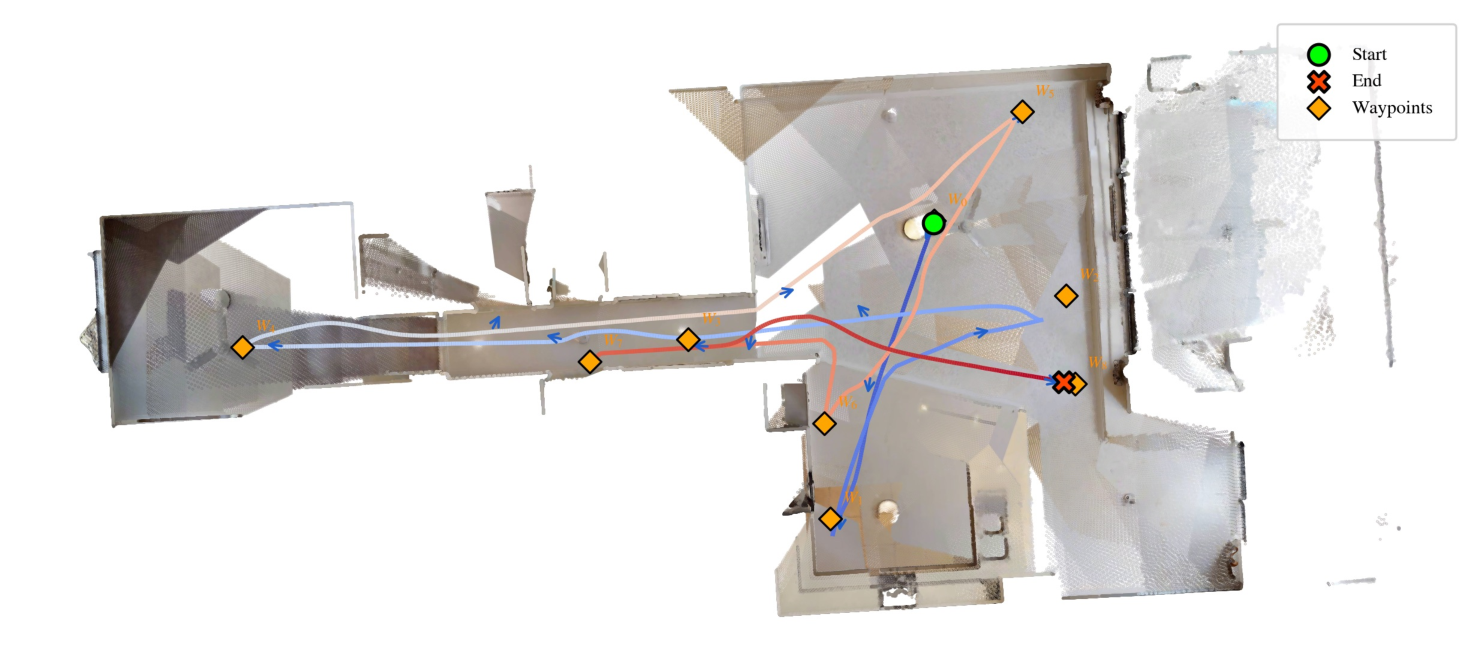
\includegraphics[height=0.2\linewidth]{figures/habitat/hm3d_1.pdf} \\[2pt]
    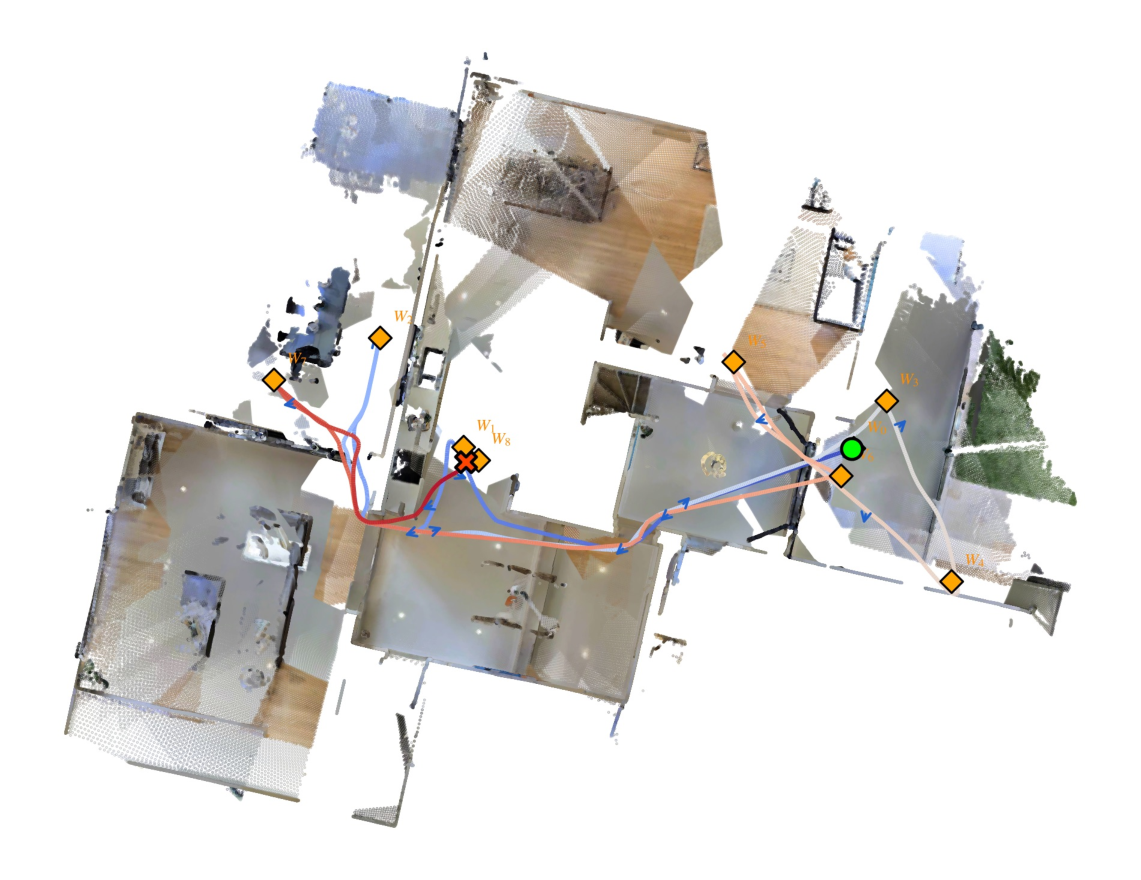
\includegraphics[height=0.2\linewidth]{figures/habitat/mp3d_2.pdf} &
    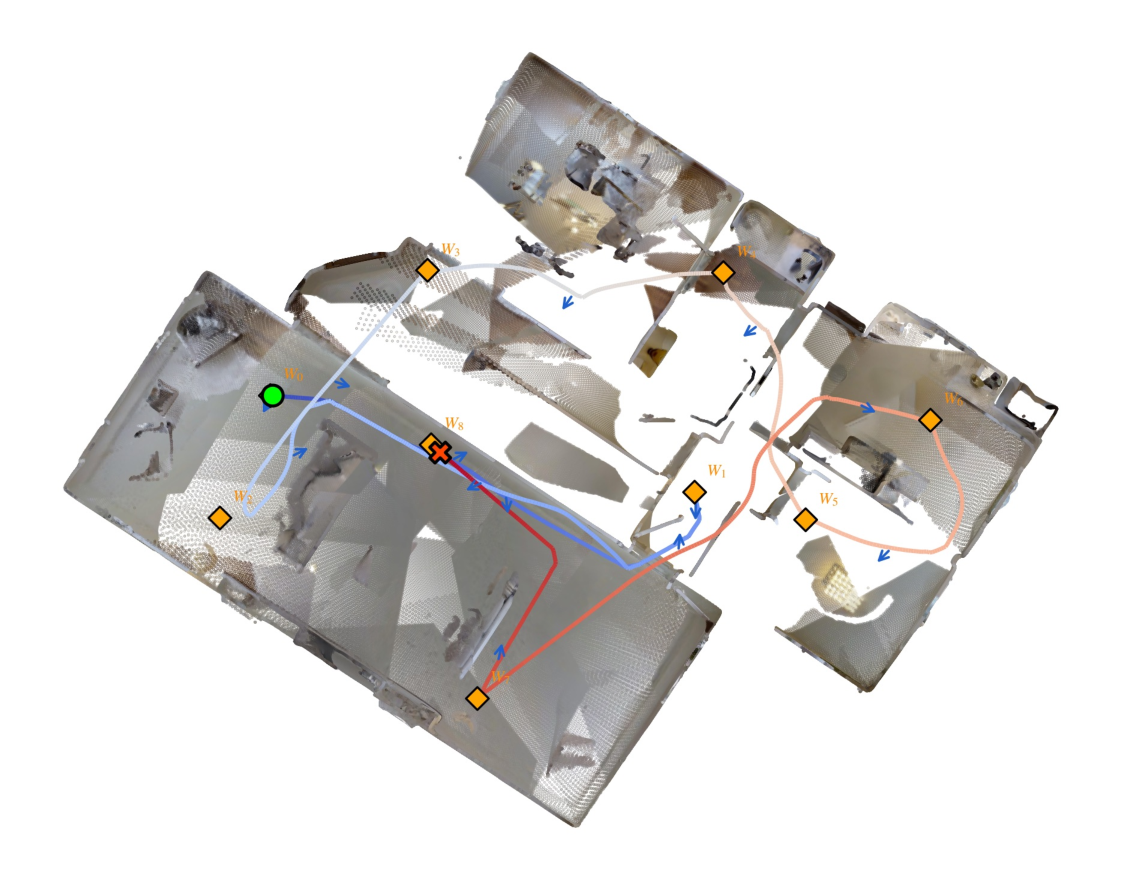
\includegraphics[height=0.2\linewidth]{figures/habitat/gibson_2.pdf} &
    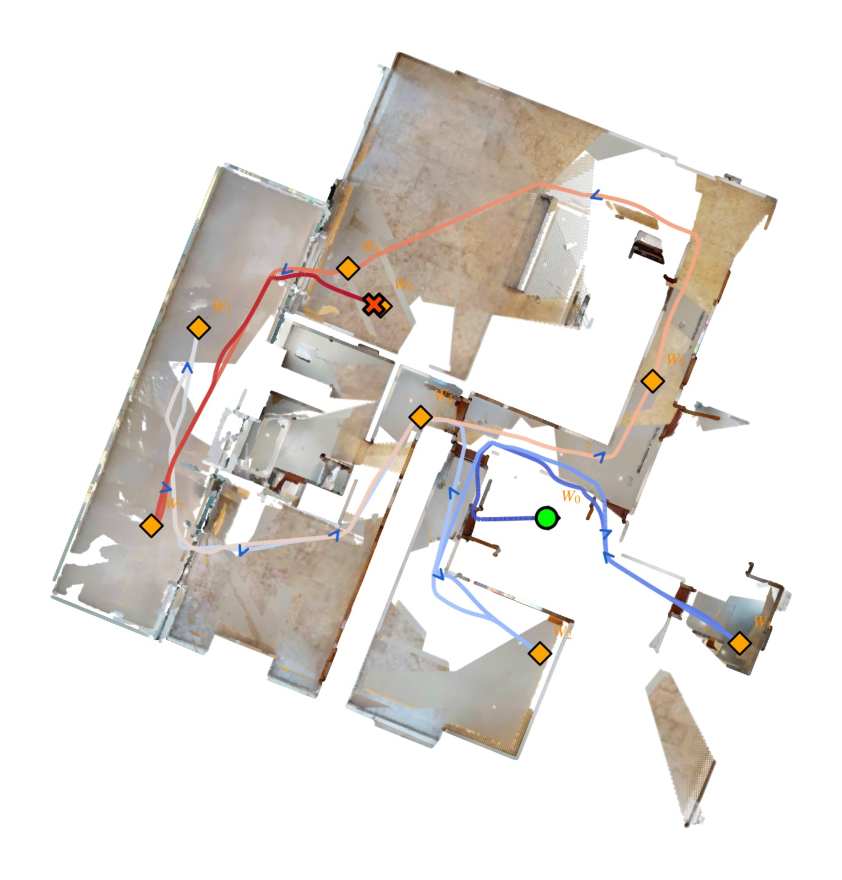
\includegraphics[height=0.2\linewidth]{figures/habitat/hm3d_2.pdf} \\[2pt]
    {\small Matterport3D} & {\small Gibson} & {\small HM3D} \\
  \end{tabular}}
  \caption{%
    Top-down visualizations of rendered point clouds and sampled camera trajectories across six scenes from three datasets (Matterport3D, Gibson, and HM3D).
    Each point cloud is colored using per-pixel RGB values from the rendered frames.
    The trajectory color varies from \textcolor{blue}{blue} (start) to \textcolor{red}{red} (end), indicating temporal progression.
    \textcolor{green}{Green} circles and \textcolor{red}{red} crosses mark the start and end positions, respectively.
    \textcolor{orange}{Orange} diamonds denote randomly sampled waypoints on the navigation mesh, and \textcolor{blue}{blue} arrows indicate the camera viewing direction at regular intervals.
  }
  \label{fig:traversal_viz}
\end{figure*}
